\documentclass[]{scrartcl}
\usepackage{graphicx}
\usepackage{color}
\usepackage[ngerman]{babel}
\usepackage{hyperref}
\usepackage{fullpage}
\usepackage{calc} 
\usepackage{enumitem}
\usepackage{titlesec}
\newcommand{\todo}[1]{\textcolor{red}{TODO: #1}\PackageWarning{TODO:}{#1!}}
\begin{document}

\title{
	\includegraphics*[width=0.75\textwidth]{images/hu_logo.png}\\
	\vspace{24pt}
	Einf"uhrung in die Sprachphilosophie}
\subtitle{VEV WS 16/17\\
          Dr. Jasper Liptow\\
          Philosophisches Institut I \\ 
          Humboldt Universit"at zu Berlin}
\author{Lennard Wolf\\
        \href{mailto:lennard.wolf@student.hu-berlin.de}{lennard.wolf@student.hu-berlin.de}}
\maketitle
\begin{abstract}

Die Vorlesung soll grundlegendes Wissen "uber Probleme, Begriffe und Positionen der Sprachphilosophie des 20. Jahrhunderts vermitteln. Nach einer einf"uhrenden Einheit, in der das Ph"anomen der sprachlichen Bedeutung, das im Mittelpunkt sprachphilosophischer Untersuchungen steht, herausgearbeitet wird, widmen wir uns ausgew"ahlten systematischen Themen (wie etwa den verschiedenen Dimensionen sprachlicher Bedeutung, dem Zusammenhang von Bedeutung und Gebrauch sprachlicher Ausdr"ucke oder dem Verh"altnis von Sprache und Denken). Die Vorlesung wird von Tutorien begleitet, in denen Texte besprochen werden, die f"ur die Vorlesung eine Rolle spielen, und Fragen der Vorlesung vertieft diskutiert werden k"onnen.


\end{abstract}
\newpage

\tableofcontents
\listoffigures
\newpage


\section{Einf"uhrungssitzung\\(24.10.16)}
\subsection{Organisatorisches}

\begin{itemize}
  \item Jede Woche begleitender Text der vorher zu lesen ist (bis 30.11. können runtergeladen werden)
  \item In Tutorien werden Texte nachbesprochen
  \item 4 Essays (3-4 Standardseiten) f"ur Tutorien zum Bestehen 
  \item Passwort: Platte
\end{itemize}

\subsection{Was ist Sprachphilosophie?}
\subsubsection{Was ist eine philosophische Methode zur Untersuchung der Sprache?}
\begin{itemize}
  \item Ziel: Erkentnisse über Sprache zu gewinnen ohne Empirie anzuwenden
  \item Philosophische Fragen sollen \emph{verschwinden}
  \item Unterschiede zu Empirischer Forschung sind umstritten (Zwei M"oglichkeiten):
  \item \textbf{Unterschiede sind prinzipieller Natur:}
  \item Empirische Wissenschaft untersucht die Welt \emph{direkt}, Philosophie durch eine Analyse unserer Begriffe
  \item Art der Rechtfertigung: a priori vs a posteriori
  \item Art der Belege: Erfahrung vs. Intuition
  \item Modaler Status des Wissens: kontingente Wahrheiten (Empirie) vs notwendige Wahrheiten (Philosophie)
  \item \textbf{Unterschiede sind gradueller Natur:}
  \item 
\end{itemize}

\subsubsection{Welche Aspekte der Sprache sind Gegenstand?}

\begin{itemize}
  \item
  \item
\end{itemize}

\newpage



\section{Frege: "Uber Sinn und Bedeutung\\(31.10.16)}

\subsection{Vornotizen zum Text}
\subsubsection{Inhalt des Textes}
\begin{itemize}
  \item \emph{R"atsel}: Wie kann $a = b$ einen anderen Erkenntniswert als $ a = a$ haben wenn es wahr ist? $\rightarrow$ \emph{Sinn} 
  \item Zeichen (Eigenname) $\rightarrow$ Sinn (das \emph{Gemeinte}) $\rightarrow$ Bedeutung (\emph{Auf das gedeutet wird})
  \item \textbf{Beispiel} -- \emph{Zeichen}: Abendstern $\rightarrow$ \emph{Sinn}: ein bestimmtes Himmelsgestirn $\rightarrow$ \emph{Bedeutung}: Venus 
  \item Bei dem Zeichen \emph{Morgenstern} w"are die Bedeutung ist identisch, aber der Sinn w"are m"oglicherweise ein anderer
  \item Der Sinn eines Eigennamens ist die \emph{Art des Gegebensein}.
  \item Der Sinn eines Satzes ist der \emph{Gedanke} (objektiver Inhalt der nicht ein Prozess in einem Kopf ist sondern von vielen gedacht werden kann) den er ausdr"uckt.
  \item Die Bedeutung eines Satzes ist sein Wahrheitswert.
  \item \emph{Das Streben nach Wahrheit also ist es, as uns "uberall vom Sinn zur Bedeutung vorzudringen treibt.}
  \item Das Urteil ist der Fortschritt von einem Gedanken zu seinem Wahrheitswert
\end{itemize}
\subsubsection{Fragen}
\begin{itemize}
  \item Ist Bedeutung nur in realer Welt (kontextunabh"angig) oder kann in zB einem literarischen Kontext eine Bedeutung vorhanden sein? (kontextsensitiv, Stichwort Odysseus)
\end{itemize}

\subsection{The Linguistic Turn }

20. Jahrhundert als Jahrhundert der Sprachphilosophie
\begin{itemize}
  \item Sprache als zentraler Gegenstand philosophischer Untersuchung
  \item K"onigsdisziplin in versch. Jhdt. unterschiedlich (z.B. Ontologie, Epistemologie etc.)
\end{itemize}

\subsection{Die Grundfrage der Sprachphilosophie}

\subsection{Bedeutung als Vorstellungen}

\subsection{Bedeutung als objektive Gegenst"ande}

\subsection{Freges R"atsel}

\subsection{Frege "uber Sinn$_{F}$ und Bedeutung$_{F}$ von Eigennamen}

\textbf{Wichtig:} Seite 42, Fu\ss note 2
\textbf{Wichtig:} Lesen: \emph{Der Gedanke }von Frege
\newpage
\section{"Uber den Dozenten}
Dr. Jasper Liptow absolvierte 1996 seinen Magister an der Universit"at Hamburg, promovierte in Gießen mit einer Arbeit zum Thema \emph{Gebrauchstheorien der Bedeutung} bei Prof. Martin Seel und ist Privatdozent.


\begin{figure}[]
	\centering
	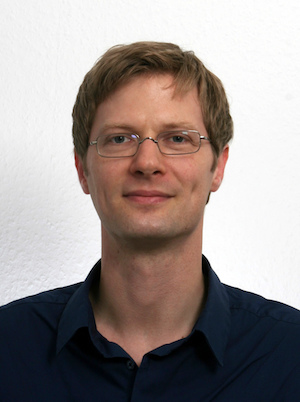
\includegraphics[width=0.32\textwidth]{images/liptow.jpg}
	\caption{Dr. Jasper Liptow. Quelle: \url{https://www.uni-frankfurt.de/45457854/liptow.jpg}}
	\label{fig:liptow}
\end{figure}

%\begin{figure}[h]
%	\centering
%	
\includegraphics[width=0.5\textwidth]{images/template.png}
%	\caption{Template Bild}
%	\label{fig:template}
%\end{figure}

\end{document}
